\chapter{Entwicklung des Prototyps}
\label{ch:development}

Die Umsetzung des Prototyps erfolgt in mehreren Schritten. Zu Beginn wird wie in \ref{sub:unifiedList} beschrieben, die Liste aller Ergebnisse zusammengeführt und absteigend nach der Relevanz sortiert. Anschließend wird der Schlagwortabgleich (\ref{sub:keyword}) implementiert, indem konfigurierbar die Liste der möglichen Synonyme mit dem Suchterm abgeglichen wird und die Ergebnisse geboostet werden, wenn der Suchterm ein Synonym enthält. Zuletzt werden die resultierenden Inhalte nach einem möglichen Vorschlag wie in \ref{sub:suggestion} beschrieben dem Ergebnis hinzugefügt.

\section{Zusammengeführte Liste}
\label{sec:devUnifiedList}

Für die Entwicklung der zusammengeführten Liste im Crossload Frontend ist wichtig, dass die schon implementierte Funktionalität der Suche nach Kategorien nach der Entwicklung immer noch möglich sein muss.
Dazu finden sich auf der Suchergebnisseite mehrere Tabs, bei denen auch eine Suche innerhalb von Kategorien möglich ist.
Sie wird angeführt von der gemischten Suchergebnisseite, auf der wir momentan die Aufteilung in verschiedene Kategorien sehen (\ref{fig:crossloadSuche}).

\begin{figure}[h]
  \begin{centering}
    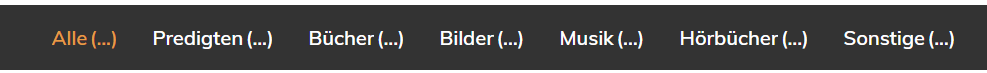
\includegraphics[width=\textwidth]{figures/development/kategorienLeiste.png}
    \caption{Leiste der Suchergebnisse in den verschiedenen Kategorien \cite{pfleiderer2022}.}
    \label{fig:kategorienLeiste}
  \end{centering}
\end{figure}

Ziel ist es, die gemischte Suchleiste so zu ändern, dass eine große Liste mit allen Kategorien gemischt angezeigt wird.
Dazu wird die bisherige Implementation wie folgt geändert:

Anstatt nach Ergebnissen pro Kategorie abzufragen und diese in den einzelnen Sektionen darzustellen, muss eine gesammelte Anfrage an die Such API gesendet werden.
Diese wird nach dem gegebenen Sortierkriterium, in diesem Fall absteigend nach Relevanzscore sortiert von der Such API zurückgegeben.
Dafür wird zu den vorhandenen Kategorien eine „gemischte“ Kategorie hinzugefügt, bei welcher dann kein Suchfilter mitgegeben wird.
Danach sind nur noch kleine Änderungen notwendig, um das für den Nutzer schön dargestellt zu bekommen.

\begin{lstlisting}[language=Java, title={Erstellen der gemischten Kategorie \cite{frontend2022}}]
  export const MIXED_RESULTS_OPTION = {
    category: "mixed",
    path: RESULTS_BASE_URL + "/gemischt",
    lastPathSegment: "gemischt",
    text: "Alle",
    longText: "Alle",
  } as const
\end{lstlisting}

\begin{lstlisting}[language=Java, title={Löschen der Kategorie aus den API Parametern \cite{frontend2022}}]
  if (category === "mixed") {
    delete url.category
  }
\end{lstlisting}

Das Ergebnis zeigt eine zusammengeführte Liste, die komplett nach Relevanz sortiert ist (\ref{fig:crossloadSucheNeu}).
Mithilfe der Symbole, die bereits bei den Ergebnissen die Kategorie bereits kennzeichneten, kann der Nutzer einfach erkennen, welcher Inhalt von welcher Kategorie ist.

\section{Schlagwortabgleich}
\label{sec:devKeywords}

Für den Schlagwortabgleich werden die Synonyme in Java konfiguriert.
Dazu wird eine Enumeration erstellt, die eine Liste der Synonyme enthält (\ref{code:SermonCategory}).
Durch diese Enumeration können Änderungen leicht eingebaut werden und durch die vorhandene \gls{ci}/\gls{cd} Pipeline direkt in die produktive Umgebung eingespielt werden.
Somit wäre der Nachteil der fest definierten Synonyme ausgeglichen, da Korrekturen schnell eingespielt werden können.

Eine Alternative zur Konfiguration in Java wäre eine ausgelagerte \gls{json} Datei.
Da diese aber genau wie die Java Enumeration, durch die CI/CD Pipeline, in die produktive Umgebung gelangen würde, wäre kein großer Nutzen dabei, eine JSON Datei der Enumeration vorzuziehen.
Der Unterschied dabei ist aber die Komplexität beim Einlesen der Datei und die fehlende Typisierung in der JSON Datei.
Aus diesem Grund wurde sich für die Enumeration entschieden.

Der nächste Schritt ist der Vergleich des Suchterms mit den verfügbaren Synonymen.
Dazu wird überprüft, ob dieser ein Synonym komplett enthält.
Damit sind auch Sonderfälle wie der Plural oder Beugungen enthalten, da für mögliche Spezialfälle bereits Synonyme in die Listen eingefügt wurden.

Für die Überprüfung werden Java Streams benutzt.
Diese machen den Source Code lesbarer und kleiner, da viele Kontrollstrukturen wegfallen.
Mithilfe der vorhandenen Klasse CrossloadCriteriaBuilder werden alle Inhalte der gefundenen Kategorie geboostet.
Für Predigten wird hierbei noch für den Spezialfall der Predigt mit Video unterschieden, bei nur Predigten mit Video geboostet werden und andere Predigten keine besondere Behandlung erfahren.

\clearpage
\begin{lstlisting}[language=Java, title={Code für Überprüfung und Boosten der Kategorien. \cite{solr-search2022}}]
  private void addCategoryBoost(String searchTerm, SolrQuery query) {
    SermonCategory.getAllCategories()
      .stream()
      .filter(category -> category.hasCategory(searchTerm))
      .forEach(category ->  {
        CrossloadCriteriaBuilder instance = CrossloadCriteriaBuilder.getInstance();
        if(SermonCategory.VIDEO.equals(category)) {
          // Boost for Sermons with video
          instance.addCriteria(SchemaField.HAS_PRIMARY_VIDEO, "true", 75);
        }
        else {
          // Boost of found category
          instance.addCriteria(SchemaField.MAIN_CAT, category.getId(), 75);
        }
        query.addCriteria(instance);
      });
  }
\end{lstlisting}

Durch das hier verfügbare Skript werden nun die Kategorien anhand des gegebenen Suchterms geboostet.

\section{Vorschläge für weitere Navigation}
\label{sec:devSuggestions}

Für die Vorschläge sind Anpassungen sowohl in Suche, um den Vorschlag herauszuarbeiten, als auch im Frontend, um den Vorschlag anzuzeigen, notwendig.

In der Such API wird hierfür zunächst die zurückgegebene Antwort um ein Vorschlagsobjekt ("suggestion") erweitert (\ref{code:SolrResponse}).
In diesem Objekt wird für das Frontend entweder die vorgeschlagene Predigt stehen, oder kein Wert, wenn es keinen Vorschlag gibt.

Um einen Vorschlag zu finden, müssen die relevantesten Inhalte nach den bereits erwähnten Kriterien untersucht werden (\ref{sub:suggestion}).
Im derzeitigen Code wird immer nur eine Suchseite mit bis zu 20 Ergebnissen zurückgegeben.
Wenn diese benutzt werden, würde um das relevanteste Ergebnis zu finden, würde man maximal einen Vorschlag pro Seite bekommen.
Dieser wäre von Seite pro Seite unterschiedlich.

Mit SOLR ist es allerdings möglich, eine Query mit einem Ergebnis und den gleichen Suchparametern abzugeben, die nur die ersten 10 Elemente einer nach dem Relevanzscore absteigend sortierten Liste zurückgibt.

\clearpage
\begin{lstlisting}[language=Java, label={code:SOLRSuggestionQuery}, title={SOLR Query für die Top 10 Ergebnisse, absteigend sortiert nach Relevanz \cite{solr-search2022}}]
  final JsonQueryRequest suggestionQuery = new JsonQueryRequest(params)
    .withParam("q", solrQuery.getQuery())
    .withParam("fl", "*, [child limit=100]")
    .withParam("rows", 10) // Get only 10 values
    .withParam("start", 0) // Start at the beginning, always
    .withParam("sort", "score desc,main_id desc");
\end{lstlisting}

Diese gefundenen Ergebnisse werden dann untersucht, um einen Vorschlag zu finden. Das Ergebnis (ein Inhalt oder \emph{null}) wird dann dem zurückgegebenen Ergebnis mitgegeben.

\begin{lstlisting}[language=Java, label={code:parseSuggestion}, title={Relevanteste Inhalte nach einem Vorschlag durchsuchen \cite{solr-search2022}}]
  public Sermon parseSuggestion(List<Sermon> mostRelevant) {
    // Case 0: If there is only one content in the list, return that as suggestion
    boolean onlyOneElement = mostRelevant.size() == 1;

    // Case 1: Score of the first element is at least twice as much of the second score
    boolean biggerThanDoubleTheScore = mostRelevant.size() > 2 && mostRelevant.get(0).getScore() >= 2 * mostRelevant.get(1).getScore();

    if(onlyOneElement || biggerThanDoubleTheScore) {
      return mostRelevant.get(0);
    }

    // Case 2: Get the average of the most relevant sermons and check if the first has at least twice as much of that
    if(!mostRelevant.isEmpty()) {
      Float average = (float) mostRelevant
        .stream()
        .mapToDouble(sermon -> sermon.getScore())
        .summaryStatistics()
        .getAverage();

      if(mostRelevant.get(0).getScore() >= 2 * average) {
        return mostRelevant.get(0);
      }
    }

    return null;
  }
\end{lstlisting}


\clearpage
Im Frontend müssen nun ebenso die Änderungen in den verschiedenen Typen gemacht werden, damit die Vorschläge auch ausgelesen werden können.
Für die Anzeige wird dann die bereits verfügbare Liste der gefundenen Inhalte verwendet um doppelten Code zu minimieren und den Vorschlag direkt anzuzeigen.


\begin{figure}[h]
  \begin{centering}
    
\includegraphics[width=\textwidth]{figures/development/suggestion.png}
    \caption{Anzeige des Vorschlags \cite{pfleiderer2022}.}
    \label{fig:suggestion}
  \end{centering}
\end{figure}


\begin{lstlisting}[language=Java, label={code:suggestionRow}, title={Code für Anzeige des Vorschlage \cite{frontend2022}}]
  <div role="rowgroup" attr.data-cy="category_suggestion">
    <app-content-list-header text="Vorschlag"></app-content-list-header>

    <app-content-list
      [contents]="[response.suggestion]"
      [maxVisible]="maxCategoryResults"
    ></app-content-list>
  </div>
\end{lstlisting}
